\subsection{Episode 64: At Dawn We Plan!}

\DndDropCapLine{I} am a monster, a foul debaser who is unsafe a companion for any creature large or small. The animal inside, is as big as the one seen from the outside. If I had been born a short stack, then at least others could have contained me, but the years of training have only honed my will and ability to maintain my own freedom. As I walk through this valley, I must take a look at myself and either fade away in inevitable decline or hope something larger takes me. Either way these new colleagues of mine will be safer for my absence.\medskip

As I stand alone on the prow of the ship, these birds will not leave me alone. I hear the inner screams of my own torment. Until what’s this another sound, one more distant. I see screaming and hear people running. This is a crisis situation, I take hold of this majestic boat and wheel it around hard. This people might need me, the might need a hero, could this be the dulcet tones of redemption. There is little time to adjust to these new surrounds, I dash into the church which seems to be at the center of this disquiet. I am met by what I will always refer to as that sight. My until recent comrades are bathed in the blood, with civilians carved up and dead all around them. I take stock, it seems clear that they have massacred these people. “Until recently I almost killed you” its a strong opener, but Myron keeps his weapon in hand, I can’t contain it, it rises up like a bile in my gut, the blood of the innocents has been spilt on these grounds, all other targets are unarmed and shocked, Myron looks to still be hostile and either confused or un-repentent. There will either be time later, or there won’t neither matter now.\medskip

Burnie jumps between us and tries to break us, Myron then talks of escape as the story, Burnie tries to talk them out of it. The marching sounds get louder, I need to buy time for the forces to arrive, these miscreants must be apprehended. As they try to walk away I run around to bar their way again.\medskip

Exmerah is in deep shock, vomiting around the bodies littered with holes. Its an impasse, as I feel the hormones running amok within my system. I cannot stand for this….\medskip

A thundering yet uninterested voice calls through the halls of the church asking for us all to render ourselves to justice.\medskip

Exmerah goes for the easy way out, I understand, we have all done things that are hard to live with, and oftentimes it would seem the easier way out would be death, but it is not. Not on my watch. It is intense as Myron and Exmerah bicker it out, their eyes fall to the body of an official on the floor with a huge hole in him.\medskip

Myron ask Exmerah if she killed these people because she was ensorcelled. Burnie and Myron are clearly looking for exits, they must answer for the crimes committed here. Myron makes a run for it up some stairs and onto a balcony. He is a lost cause but I can still do the right thing here. I walk out pushing the remaining doors wide open, I state my name and cause and drop to my knees in surrender in front of the arbiters.\medskip

Myron breaks out of the roof, and Exmerah sends out the giant robot to treat with the arbiters.\medskip

“You have 3 seconds to come out!” the arbiter calls out and counts down, on “Go” the armed forces unleash a barage of shot, annihilating the poor robotic dog, they step in line and march into the church. A cavalcade of shot rings out as they are spotted on the balcony.\medskip

“I am Rab Burnie Cinders, and you know that name” He shouts as he takes the guns off Myron and Exmerah “I’ll kill them both”. It’s a great strat and at first seems like it might work, until Kyros notifies them that Myron isn’t a hobo but in fact a very naughty arbiter. They rush to the roof, looking for the airship, or any other way out. The pursuers close the distance in no time. Burnie appeals to Laz in a last ditch effort to escape. Exmerah pulls out the cube and in an instant all three of them are gone. “ I didn’t kill my wife” rings out where previously only the peal of bells could be heard. The whole town would care, if they weren’t mostly slaughtered below.\medskip

\textbf{---}\medskip

I announce to them who I am, and what my rank entitles me to. If I am guilty then I shall answer to the crimes, if not then I shall see them again. At this point the arbiter goes to use that word of truth on me, I have nothing to hide so I succumb, only to find myself admitting to the crimes seen here. This is something I haven’t even seen the greatest negotiators manage with such ease. Maybe the ensorcering is true, either way Kyros must have been aware that I was not in the church during the massacre.\medskip

It now seems a mute point as I am battered half to death, until I slip into a painful sleep.\medskip

\textbf{---}\medskip

The miscreant team reappear in a cupboard, Burnie suggests torturing Toni with a cucumber. Myron takes of his armour, stashing it in the magic bag of Exmes. In his new guise as normal Myron. Burnie tries to disguise himself and Exmerah, he makes a strong effort in trying to combine Myron and Exmerah into one trench coated person. It’s not a great result, and they fall back to individual disguises, luckily the house is empty and the creeping begin. Exmerah spots a family photo of a some very recently deceased people. She removes the photo, rolls it and puts it into her bag. They creep outside, Myron suggest splitting up and keeping in contact using the ear pieces. Everyone is to sneak towards where the airship should be, and then try and get into contact with Riphard. Exmerah gives them both a rocket, Myron extorts her to not get captured and not give herself up.\medskip

As they are leaving Burnie sees Toni beaten and battered being dragged away to a steel barred prison wagon. Khaan and Kyros are talking shit about where the airship is, apparently it took off into the sky, but she is sure it will be back. Burnie adds a new boot to his peg leg, in an attempt to make it less obvious who he is. He used the communicator to contact the barely conscious cat.\medskip

I lure him closer with talk about the ear-piece that I am wearing. As he comes in to inspect and reaches his arm into the cage, I grab his arm and break it across the bars of the cage, I then grab his face and bounce his head against another bar. Burnie unleashes a bolt from a hidden position killing the guard instantly. I spin on my heels and pull the dead guards sword from his belt before lancing it into the guard behind me. Burni unleashes another wave of pain into the guard who then starts running and shouts for assistance. Burnie shoots a third and final bolt through the back of the head, three down. Burnie then frees me, out of all of them I would not have put money on it being Rab.\medskip

Myron sets off a rocket in a barrel of fish, as we make our escape into the woods. We converge and make our escape. I switch Burnie for Exmerah and keep running until my lungs are on fire. Myron postulates, but I need time to figure out what has taken place. Clearly something has gone amiss, Myron starts trying to explain who freyer is, but still nothing really makes sense. Why set up Myron and the rest of the group, why not kill them outright and then massacre the town. Why have Myron and the group massacre a whole village. Why does she want Godling bay. None of this makes sense.\medskip

Myron leads us further into the woods, until I am certain we are lost. Myron hands out some jerky that is surprisingly filling. I let the others sleep before asking the animals to watch over us as we sleep.\medskip

We wake up cold and wet, the revelations start flowing, it turns out Freyer knew the details of all the party members. Was Kyross part of the plan to frame them, where were these troops, the army was much too large for dealing with just a small SRA group.\medskip

Exmerah uses the earpieces to triangulate and boost the signal to get in touch with Riphard. Will she won’t she request the return of the airship. She requests the airship return to pick them up. The least subtle airship over a forest scenario then takes place.\medskip

There is some debate about where to head to next, Exmerah decides to invent parachutes.\medskip

It turns out that Julian Assange the arbiter ate a banana with the skin on, this led to his seeking exile in the masudan embassy for a while.\medskip

There is much discussion about what we should do, I for one would like some vengeance. We ascend above the clouds and under a dark starlit night we sleep. A war council will be formed on the morrow, At Dawn We Plan!\medskip

https://www.youtube.com/watch?v=ExLqMBLyWd8

Epilogue - Sat above in the crows nest alone once again with his thoughts and a few remaining starlings. A lone tiger looks aloft and things to himself, "They are monsters, they are foul debasers, they shall pay for what they have wrought".\medskip

\vspace*{5mm}

\begin{center}
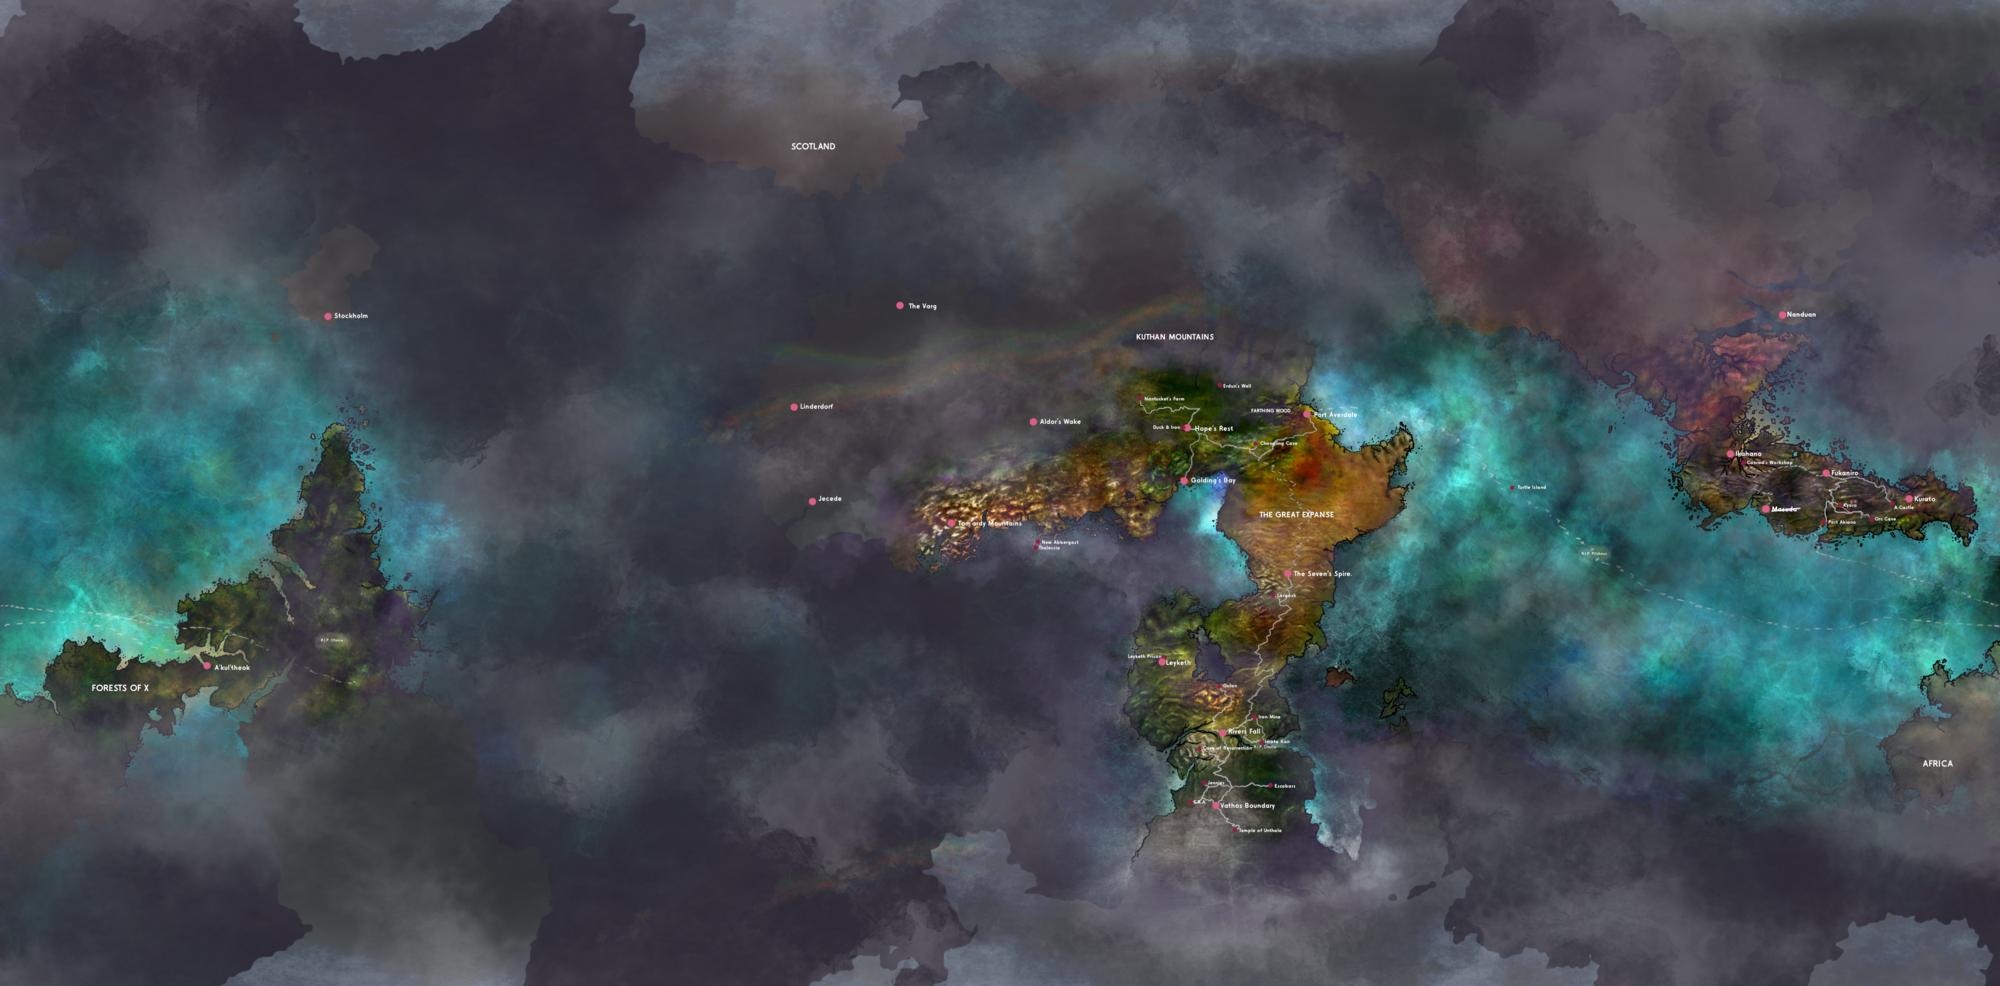
\includegraphics[width=\textwidth]{./content/img/reddit/mapEp64.png}\\
\textit{This tainted, bitter world. (Map as of Episode 64)}
\end{center}

